\documentclass{scrreprt}

\usepackage{etoolbox}
\makeatletter
\patchcmd{\scr@startchapter}{\if@openright\cleardoublepage\else\clearpage\fi}{}{}{}
\makeatother

%Für deutsche Trennung
\usepackage[ngerman]{babel}
%Für UTF8-Codierung, mit Umlauten!
\usepackage[utf8]{inputenc}

%Für Links, auch innerhalb des Dokuments
\usepackage{hyperref}

%Einbinden von Grafiken
\usepackage{graphicx}

\title{Anwenden der Low Level Design Patterns}
\author{Gruppe H}
\date{\today}

\begin{document}

\maketitle
\tableofcontents

\part{Welches Low Level Design Pattern eignet sich für unseren Faithinator?}

\chapter{Client-Dispatcher-Server (CDS)}
Da dieses Pattern hauptsächlich von den zentralen Rolle des Dispatchers abhängt, der allerdings das Interface für die Clients darstellt, wären künftige Anpassungen am Interface äußerst komplex und risikoreich. Die großen Vorteile dieses Patterns (Server-Redundanz, geringer Migrationsaufwand, Fehlertoleranz) sind für unseren Faithinator nicht die wichtigsten Eigenschaften. Hier wären eher Erweiterbarkeit und Wartbarkeit zu nennen.

\chapter{Command Processor}
Das Command-Processor Pattern eignet sich (fast) ausschließlich zur Protokollierung von Ereignissen (d.h. bspw. Erstellung von Logs oder Ermöglichen des Undo-Befehls). Daher eignet es sich denkbar schlecht für unseren Faithinator.

\chapter{Forwarder Receiver}
Das Design Pattern "Forwarder Receiver" ist ebenfalls nicht geeignet für unsere Applikation. Es bietet eine Peer-to-Peer Kommunikation, sodass verschiedene Knoten in einem Netzwerk kommunizieren können. In unserer App sollen gibt es jedoch eine zentralen Server, auf dem alle Anfragen bearbeitet und alle Daten gespeichert werden.

\chapter{Master-Slave}
Das Master-Slave Pattern wird genutzt um Arbeit zu partitionieren, dies wird zum Beispiel genutzt um Probleme mit langer Laufzeit zu lösen. Im Fall unseres Faithinators ist dies nicht der Fall, somit ist es nicht sinnvoll das Master-Slave Pattern anzuwenden.

\chapter{Proxy}
Das Proxy Pattern lässt sich gut für unseren Faithinator nutzen. Da es eine Zwischeninstanz zwischen Clients und Original bildet um direkte Kommunikation zu vermeiden. In unserem Fall könnte das Proxy Pattern einen Übergang zwischen Clients/Admins und der Datenbank bilden. Damit kann sichergestellt werden ,dass die Clients und Admins nicht unbegrenzten Zugriff auf die Datenbank haben.
\begin{figure}[ht]
 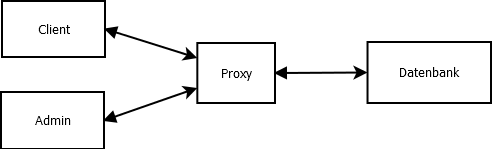
\includegraphics[width=\textwidth]{./pics/Proxy.png}
 % Diagramm1e.eps: 0x0 pixel, 300dpi, 0.00x0.00 cm, bb=0 0 765 425
 \caption{Übersicht: Zusammenarbeit der Komponenten beim Proxy-Pattern}
 \label{abb:1}
\end{figure}

\chapter{Publisher Subscriber}
Das Publisher-Subscriber-Pattern würde sich dazu eignen, das Versenden der Fragen an die Clients zu verwalten. 
Clients können sich dafür entscheiden, an einer angebotenen Fragestellung teilzunehmen, in diesem Fall können sie beim Publisher (Server) als Subscriber eingetragen werden. Der Publisher kann dann Benachrichtungen zum Start oder Ende der Fragezeit und den Chatrunden verteilen.
Wenn Einladungen zu Fragen zielgruppenspezifisch versendet werden sollen, ließe sich das ebenfalls über dieses Pattern realisieren, ebenso wie ein Benachrichtigungssystem für die Admins einer Frage.

\chapter{View Handler}
Das Design Pattern "View Handler" ist für unsere Applikation nicht notwendig oder von Vorteil. Es gibt für jede Aktion eine eigene grafische Benutzeroberfläche, Daten müssen nicht in verschiedenen Fenster in verschiedenen Formaten dargestellt werden. Das Potenzial des View Handler Patterns würde nicht genutzt werden.

\end{document}
